% ICML 2025 Paper Template for Overleaf
% Auto-generated by Anonymous Research Pipeline — Phase 6.5.1
%
% Instructions:
% 1. Upload this folder to Overleaf
% 2. Ensure icml2025.sty is in the same directory
% 3. Compile with pdfLaTeX
%
\documentclass{article}

% ICML 2025 style - download from https://icml.cc/Conferences/2025/StyleAuthorInstructions
\usepackage{icml2025}

% Standard packages
\usepackage{microtype}
\usepackage{graphicx}
\usepackage{booktabs}
\usepackage{hyperref}
\usepackage{amsmath}
\usepackage{amssymb}
\usepackage{algorithm}
\usepackage{algorithmic}

% For better table formatting
\usepackage{multirow}
\usepackage{makecell}

% Bibliography
\usepackage{natbib}

% ============================================================================
% DOCUMENT METADATA
% ============================================================================

\icmltitlerunning{Symmetry Orbits Are Geometrically Large in MLP Weight Spaces}

\begin{document}

\twocolumn[
\icmltitle{Symmetry Orbits Are Geometrically Large in MLP Weight Spaces: Implications for Weight Space Encoding}

% Author information - fill before submission
\icmlsetsymbol{equal}{*}

\begin{icmlauthorlist}
\icmlauthor{Anonymous Author}{inst1}
% \icmlauthor{Author Two}{inst1,inst2}
% \icmlauthor{Author Three}{inst2}
\end{icmlauthorlist}

\icmlaffiliation{inst1}{Anonymous Institution, City, Country}
% \icmlaffiliation{inst2}{Second Institution, City, Country}

\icmlcorrespondingauthor{Anonymous Author}{anonymous@anonymous.org}

\icmlkeywords{Machine Learning, ICML, weight space learning, symmetry, canonicalization, neural functional transformer}

\vskip 0.3in
]

% Print title but hide author info for review
\printAffiliationsAndNotice{}  % For camera-ready

% ============================================================================
% ABSTRACT
% ============================================================================

\begin{abstract}
Two neural networks can compute the same function yet occupy nearly orthogonal positions in weight space --- a geometric reality with concrete consequences for any method that learns from raw neural network weights. We provide the first empirical quantification of scaling and sign-flip symmetry orbit diameters as cosine distances in a real MLP model zoo, finding that both symmetry types produce geometrically large orbits (mean cosine distances 0.32 and 1.07, respectively; 100\% of oracle-constructed pairs exceed the significance threshold). We then probe whether the Neural Functional Transformer (NFT), a state-of-the-art permutation-equivariant encoder, is naturally invariant to these orbits. The result is asymmetric: NFT is measurably non-invariant to scaling orbits (embedding gap $+0.024$, 95\% CI$=[0.023, 0.025]$) but approximately invariant to sign-flip orbits by construction --- an emergent consequence of its row-level tokenization, not a deliberate design choice. We further show that the standard majority-sign canonicalization algorithm fails to produce a unique canonical form for 85.6\% of models in the zoo, due to an arithmetic property of even input dimension that the literature has not previously characterized. Together, these findings transform the argument for symmetry canonicalization from a theoretical expectation into a measurement-grounded framework that specifies which symmetries require preprocessing, which standard algorithms fail and why, and what experimental scale is needed to detect the downstream improvement.

\end{abstract}

% ============================================================================
% MAIN CONTENT
% ============================================================================

\section{Introduction}

Two neural networks can compute the exact same function yet occupy nearly orthogonal positions in weight space --- separated by a mean cosine distance of 1.07, nearly as large as two random unrelated vectors. This is not a corner case: every oracle-constructed sign-flip orbit pair we measure ($N=2{,}500$ total, comprising 5 conditions $\times$ 500 pairs each) exceeds the geometric significance threshold of 0.05 cosine distance. Scaling orbits add a second dimension of the same problem --- mean cosine distance 0.32, again 100\% above threshold.

Weight space learning --- predicting model properties, enabling model merging, supporting continual learning --- depends on encoders that extract meaningful geometric structure from neural network weights. But if two functionally identical networks occupy diametrically opposite positions in weight space, any method operating on raw weights must either learn to ignore this variation or waste representational capacity tracking it. The dominant paradigm, permutation-equivariant encoders \citep{Zhou2023, Navon2023}, addresses the relabeling symmetry of neurons but leaves scaling and sign-flip symmetries --- which theory shows are equally well-defined for ReLU MLPs \citep{Navon2023EquivariantArchitectures} --- empirically uncharacterized in real model zoos.

This paper provides the first empirical quantification of scaling and sign-flip orbit diameters as cosine distances in a real model zoo --- distinct from prior empirical work \citep{Entezari2022, Ainsworth2022} which characterizes permutation symmetry but not scaling or sign-flip orbit geometry.\footnote{Entezari et al.\ \citep{Entezari2022PermutationSymmetry} and Ainsworth et al.\ \citep{Ainsworth2022GitReBasin} characterize the geometry of permutation symmetry orbits in the context of model merging. Schürholt et al.\ \citep{Schurholt2022ModelZoos} characterize statistical properties of model zoo populations. Neither measures the cosine distance diameter of scaling or sign-flip orbits in a real zoo, which is our specific contribution.} We measure the geometric diameter of scaling and sign-flip orbits in the Schürholt MNIST model zoo \citep{Schurholt2022ModelZoos}, a benchmark of 2-layer MLPs with ground-truth property labels. We then probe whether a state-of-the-art equivariant encoder, the Neural Functional Transformer (NFT) \citep{Zhou2023NeuralFunctionalNetworks}, is naturally invariant to these orbits --- and whether explicit canonicalization helps. The answers reveal a more nuanced picture than the theoretical argument alone suggests.

\textbf{NFT is non-invariant to scaling orbits but approximately invariant to sign-flip orbits by construction.} For scaling-orbit pairs, NFT embeddings show within-orbit cosine similarity 0.971, significantly lower than cross-orbit same-property similarity 0.995 (gap$=+0.024$, 95\% CI$=[0.0232, 0.0245]$). For sign-flip pairs, the gap is $-0.0007$ --- 34$\times$ smaller, with within-orbit similarity actually marginally \textit{higher} than cross-orbit. NFT's row-level tokenization operates on magnitude statistics, making it inherently approximately sign-agnostic. This asymmetry was not built by design; it is an emergent property of the architecture.

The natural next step --- canonicalize weights before encoding --- runs into a structural barrier. We show that the majority-sign algorithm, the standard approach to sign-flip canonicalization for $M=2$ ReLU MLPs \citep{Navon2023EquivariantArchitectures}, produces a unique canonical form for only 14.4\% of Schürholt zoo models. For even input dimension $d_{\mathrm{in}}=784$, binomial combinatorics predict an 83\% tie rate per model (observed: 85.6\%), rendering the algorithm non-unique for the overwhelming majority. Property prediction experiments at the available zoo scale ($N=500$) are statistically underpowered --- all condition comparisons yield Spearman $\rho$ confidence intervals of width $\approx 0.6$ --- but directional estimates consistently favor canonicalization ($\Delta\rho = +0.05$--$0.08$ across all tasks). We further caution that full canonicalization (Condition D) did not outperform random normalization (Condition E) at $N=500$; we attribute this to the non-unique sign-flip canonicalization described above, but this attribution remains post-hoc pending adequately-powered follow-up.

\textbf{A note on NFT's current performance.} NFT achieves Spearman $\rho \approx 0.11$ on the Schürholt MNIST zoo at $N=500$, while layer statistics \citep{Unterthiner2020PredictingNN} achieves $\rho \approx 0.9$. This substantial gap is primarily a consequence of underpowered training ($N=400$ training samples) and reflects the invariance problem our work analyzes: NFT devotes representational capacity to tracking symmetry-induced weight variation rather than functional properties. Our canonicalization experiments are designed to close this gap at adequate $N$; the poor baseline $\rho$ motivates, rather than undermines, the invariance analysis.

We make four contributions:

\begin{enumerate}
\item \textbf{Orbit diameter measurement.} First empirical quantification of scaling and sign-flip orbit diameters as cosine distances in a real MLP zoo: scaling mean cosine distance 0.3232 (CI$=[0.3226, 0.3238]$), sign-flip 1.075 (CI$=[1.0705, 1.0789]$), both 100\% above the 0.05 threshold across 2,500 oracle-constructed orbit pairs (5 conditions $\times$ 500 pairs per condition).

\item \textbf{NFT invariance probe.} First quantification of NFT's non-invariance to scaling symmetry (gap$=+0.024$, CI$=[0.0232, 0.0245]$) and emergent approximate invariance to sign-flip symmetry (gap$=-0.0007$) --- an asymmetric result not anticipated by the architecture design.

\item \textbf{Geometric concentration.} Scaling canonicalization increases PCA explained variance ratio from 0.055 to 0.086 at $k=20$ principal components, confirming that canonicalization removes geometric redundancy even when downstream property prediction improvement cannot be detected at $N=500$.

\item \textbf{Structural limitation characterization.} Identification and quantitative characterization of the majority-sign canonicalization failure for even-$d_{\mathrm{in}}$ architectures, with a combinatorial root-cause analysis and a proposed fix (odd $d_{\mathrm{in}}$, alternative tie-breaking, or scaling-only canonicalization).
\end{enumerate}

Together, these contributions transform the argument for symmetry canonicalization in weight space learning from a theoretical expectation into a measurement-grounded framework --- one that specifies exactly which symmetries require canonicalization, which standard algorithms fail and why, and what scale of zoo is needed to detect the downstream effect.

The remainder of the paper is organized as follows. Section~\ref{sec:related} reviews the weight space learning literature and positions our contributions. Section~\ref{sec:method} describes our methodology: oracle orbit construction, NFT invariance probing, and canonicalization implementation. Section~\ref{sec:experiments} presents experimental setup. Section~\ref{sec:results} reports results across all four sub-hypotheses. Section~\ref{sec:discussion} discusses implications, limitations, and the path to adequately-powered follow-up experiments. Section~\ref{sec:conclusion} concludes.

\section{Related Work}
\label{sec:related}

\subsection{Weight Space Property Prediction}

The task of predicting held-out model properties from neural network weights was established by \citet{Unterthiner2020PredictingNN}, who showed that layer-wise statistics (mean, variance, higher moments of weight distributions per layer) achieve Spearman $\rho \approx 0.9$ on simple model zoo tasks. While remarkably effective as a baseline, layer statistics are permutation-agnostic --- they ignore the geometric structure of weight space entirely. They establish the task's feasibility but provide no information about which aspects of weight space geometry encode property-relevant information.

The \citet{Schurholt2022ModelZoos} model zoo dataset introduced a large-scale benchmark of diverse MLP populations trained with varying hyperparameters, making systematic comparison of weight space encoders possible. \citet{Schurholt2021HyperRepresentations} further proposed Hyper-Representations: self-supervised pretraining on model weight populations to learn shared representations. These methods treat weight populations as datasets for unsupervised learning but do not directly address symmetry structure.

\subsection{Equivariant and Invariant Encoders for Weights}

A theoretically principled line of work builds encoders that are \textit{equivariant} or \textit{invariant} to the symmetries of weight space. \citet{Zhou2023NeuralFunctionalNetworks} introduced Neural Functional Networks (NFN), characterizing the complete class of linear maps equivariant to neuron permutations for MLP weights. Their Neural Functional Transformer (NFT) variant applies attention over weight tokens, achieving state-of-the-art property prediction while preserving permutation equivariance. NFT achieves Spearman $\rho \approx 0.11$ on the Schürholt MNIST zoo at $N=500$ --- substantially below the layer statistics baseline ($\rho \approx 0.9$); Section~\ref{sec:experiments} contextualizes this gap as a consequence of underpowered training ($N=400$ samples) combined with NFT devoting representational capacity to symmetry-induced weight variation, which our canonicalization experiments are designed to address.

\citet{Navon2023EquivariantArchitectures} extended the theoretical analysis to the full symmetry group of MLP weight spaces, including \textit{scaling} and \textit{sign-flip} symmetries beyond permutation. For a 2-layer ReLU MLP with hidden dimension $h$, the scaling symmetry group has dimension $h$ (one free scale per hidden neuron) while the sign-flip symmetry group has order $2^h$. Navon et al.'s DWSNets architecture builds in equivariance to these additional symmetries, but is restricted to networks with $M \geq 3$ layers and is incompatible with the $M=2$ Schürholt MNIST zoo. Critically, while the theoretical characterization is complete, \textbf{no prior work has empirically measured the geometric diameter of scaling or sign-flip orbits in a real model zoo as cosine distances}, nor has any prior work probed whether existing equivariant encoders like NFT are naturally invariant to these orbits in practice.

Our work bridges this gap: we provide the first empirical orbit diameter measurements (as cosine distances) and the first mechanistic probe of NFT's symmetry handling, complementing the theoretical characterization of \citet{Navon2023EquivariantArchitectures} with data-grounded analysis.

\subsection{Symmetry and Canonicalization in Neural Networks}

The role of weight space symmetries in neural network optimization and representation has been studied from multiple angles. \citet{Ainsworth2022GitReBasin} showed that permutation symmetry can be exploited via ``Git Re-Basin'' to reduce loss barriers between independently trained networks, suggesting that permutation orbits have significant geometric diameter in practice. \citet{Entezari2022PermutationSymmetry} proved that, with permutation alignment, loss barriers between networks approach zero under mild conditions. These results motivate orbit-aware processing but focus on permutation, not scaling or sign-flip.

Symmetry canonicalization as a preprocessing step has been proposed in the context of molecular geometry (where canonical atom orderings improve learning) and 3D point clouds (where SO(3) canonicalization removes rotational ambiguity). In weight space, canonicalization was proposed theoretically by \citet{Navon2023EquivariantArchitectures} but not empirically evaluated for property prediction. Our work provides the first such evaluation, including a structural limitation analysis of the majority-sign algorithm that has not appeared in prior literature.

\subsection{Model Zoo Benchmarks}

\citet{Kofinas2024UniversalNeuralFunctionals} proposed Universal Neural Functionals (UNF), extending equivariant processing across architectures. While UNF addresses the cross-architecture generalization gap, it still operates on raw weights without addressing scaling or sign-flip canonicalization. Our work is orthogonal: canonicalization is a preprocessing step applicable to any encoder, including UNF and NFT, and our probe methodology can be applied to characterize any encoder's symmetry handling.

\textbf{Positioning.} We do not compete with NFN, DWSNets, or UNF on property prediction performance. Rather, we add an empirical measurement layer that all these methods implicitly need: orbit characterization tells practitioners which symmetries require canonicalization, how large the orbits are, and whether a given encoder already handles them. For NFT specifically, our finding that sign-flip invariance emerges naturally while scaling invariance does not is immediately actionable --- it suggests that scaling canonicalization is the productive preprocessing target for NFT-family encoders.

\section{Methodology}
\label{sec:method}

Our methodology is organized around four interconnected experimental questions, each with a distinct measurement protocol. The central design principle is \textbf{oracle orbit construction}: rather than inferring symmetry structure from natural variation in the zoo, we directly construct ground-truth functional equivalents by applying explicit symmetry transforms. This provides controlled probes unavailable from zoo statistics alone.

\subsection{Setting and Data}

\textbf{Model Zoo.} We use the Schürholt MNIST model zoo \citep{Schurholt2022ModelZoos}, a collection of 2-layer MLPs trained on MNIST with architecture $784 \to 64 \to 10$ (ReLU activations, no bias in the final layer). Models vary in learning rate, weight decay, and random initialization seed. We use a locally archived subset of $N=500$ models with ground-truth property labels: test accuracy, generalization gap (train $-$ test accuracy), and learning rate recovery. Weights are stored as flat tensors of dimension $D=51{,}850$ ($784 \times 64 + 64 \times 10$).

\textbf{Why this zoo.} The $M=2$ architecture makes scaling and sign-flip canonicalization well-defined: for a single hidden layer with $h=64$ neurons, scaling orbits have dimension 64 (one free scale per neuron), and sign-flip orbits have discrete order $2^{64}$. The majority-sign algorithm for sign-flip canonicalization is unambiguous in theory for $M=2$ (only one consecutive layer pair exists). As we show, this theoretical unambiguity does not hold in practice for even $d_{\mathrm{in}}$ --- a structural finding of independent interest.

\subsection{Symmetry Orbit Construction}

\textbf{Scaling orbits.} For a 2-layer ReLU MLP with weight matrices $W_1 \in \mathbb{R}^{d_{\mathrm{in}} \times h}$ and $W_2 \in \mathbb{R}^{h \times d_{\mathrm{out}}}$, the scaling symmetry transform applies per-neuron positive rescaling:
\begin{equation}
W_1[:, i] \leftarrow \alpha_i W_1[:, i], \quad W_2[i, :] \leftarrow W_2[i, :] / \alpha_i
\end{equation}
for any $\alpha_i > 0$. The resulting network computes the same function as the original for any input. We sample scaling factors log-uniformly: $\log \alpha_i \sim \mathrm{Uniform}(\log 0.1, \log 10)$, covering a $100\times$ dynamic range per neuron.

\textbf{Sign-flip orbits.} The sign-flip symmetry transform applies per-neuron sign changes:
\begin{equation}
W_1[:, i] \leftarrow s_i W_1[:, i], \quad W_2[i, :] \leftarrow s_i W_2[i, :]
\end{equation}
for $s_i \in \{-1, +1\}$. After flipping both weight sets, the output contribution from neuron $i$ becomes $(s_i W_2[i,:])\cdot\mathrm{ReLU}(s_i W_1[:,i]\cdot x)$. For $s_i = -1$: $(-W_2[i,:])\cdot\mathrm{ReLU}(-W_1[:,i]\cdot x)$. This equals the original $W_2[i,:]\cdot\mathrm{ReLU}(W_1[:,i]\cdot x)$ exactly only when the neuron is in its linear regime. In practice, we treat sign-flip orbits as \textbf{approximate} functional equivalence classes. We sample signs uniformly: $s_i \sim \mathrm{Bernoulli}(0.5)$ mapped to $\{-1, +1\}$.

\textbf{Oracle construction.} For each base model $b$ in the zoo, we construct an oracle orbit member $b'$ by applying the transform with randomly sampled parameters ($\alpha$ or $s$). This yields 500 oracle orbit pairs per symmetry type per condition. All random seeds are fixed for reproducibility.

\subsection{NFT Invariance Probe}

\textbf{Encoder.} We use NFT \citep{Zhou2023NeuralFunctionalNetworks} with $d_{\mathrm{model}}=256$, 4 attention layers, 8 heads, and CLS-token pooling. NFT was trained on Condition A (raw weights) for property prediction, then frozen. Weights are tokenized row-by-row from each weight matrix; the CLS token's final-layer representation serves as the model embedding.

\textbf{Within-orbit vs.\ cross-orbit similarity.} For each oracle orbit pair $(b, b')$, we extract embeddings $e(b)$ and $e(b')$. Within-orbit similarity is $\cos(e(b), e(b'))$. For cross-orbit comparison, for each base model $b$ we select a different model $c$ from the zoo with the same test accuracy decile.

\textbf{Invariance gap.} We define the invariance gap as:
\begin{equation}
\text{gap} = \overline{\text{cross-orbit same-property similarity}} - \overline{\text{within-orbit similarity}}
\end{equation}
A positive gap indicates the encoder does NOT treat symmetry-related models as more similar (non-invariant). We compute bootstrap 95\% confidence intervals ($n_{\mathrm{boot}}=1{,}000$) on the gap.

\subsection{Canonicalization Conditions}

We evaluate five experimental conditions:

\begin{table}[h]
\centering
\caption{Canonicalization conditions evaluated.}
\label{tab:conditions}
\begin{tabular}{llp{5cm}}
\toprule
Condition & Preprocessing & Purpose \\
\midrule
A & Raw weights (no preprocessing) & NFT baseline \\
B & Scaling canonicalization only & Isolate scaling effect \\
C & Sign-flip canonicalization only & Isolate sign-flip effect \\
D & Scaling + sign-flip canonicalization & Full canonicalization \\
E & Random normalization control & Test normalization artifact hypothesis \\
\bottomrule
\end{tabular}
\end{table}

\textbf{Scaling canonicalization.} Per-layer L2 normalization: each hidden neuron's incoming weight vector is scaled to unit L2 norm, with the corresponding outgoing weights scaled by the inverse. This collapses all scaling-orbit members to the same canonical representative.

\textbf{Sign-flip canonicalization (majority-sign).} For each hidden neuron $i$, compute the sign majority of row $W_1[:, i]$. If more weights are negative than positive, flip: $W_1[:, i] \leftarrow -W_1[:, i]$, $W_2[i, :] \leftarrow -W_2[i, :]$.

\textbf{Random normalization control (Condition E).} Each hidden neuron's incoming weights are scaled by a random factor drawn from $\mathcal{N}(1, 0.1)$.

\subsection{Canonicalization Uniqueness Audit}

The majority-sign algorithm requires a strict sign majority per neuron. For $d_{\mathrm{in}}=784$ weights per neuron, a tie occurs when exactly 392 components are positive and 392 are negative. The binomial probability of this event is:
\begin{equation}
P(\text{tie}) = \binom{784}{392} 0.5^{784} \approx 2.8\%
\end{equation}
For $h=64$ neurons per model, the probability of at least one tie per model is:
\begin{equation}
P(\text{at least one tie}) \approx 1 - (1 - 0.028)^{64} \approx 83\%
\end{equation}
We empirically audit all $N=500$ zoo models, recording: fraction with unique canonical form, number of tied neurons per model, and idempotency verification.

\subsection{Geometric Concentration Analysis}

To test whether canonicalization concentrates property-relevant geometric structure, we apply PCA to both raw (Condition A) and canonicalized (Condition D) weight matrices. We measure:
\begin{itemize}
\item \textbf{Explained Variance Ratio (EVR)} at $k \in \{10, 20, 50\}$ principal components.
\item \textbf{Linear regression $R^2$} from top-$k$ PCs onto each property label, with bootstrap 95\% CIs.
\end{itemize}

\subsection{Property Prediction Experiments}

\textbf{Protocol.} For each condition (A--E), we train NFT from scratch as a property predictor on the 400 training models ($N=500$ zoo, 80/10/10 split: 400 train, 50 validation, 50 test). Hyperparameters: Adam optimizer, lr$=10^{-3}$, weight\_decay$=10^{-4}$, max\_epochs$=50$, early stopping on validation Spearman $\rho$ (patience$=10$). Evaluation: Spearman $\rho$ on the 50-model held-out test split, averaged across 3 random seeds.

\textbf{Statistical analysis.} Bootstrap 95\% CIs ($n_{\mathrm{boot}}=1{,}000$) on Spearman $\rho$ and condition differences ($\Delta\rho$). At $n=50$ test samples, CI width for Spearman $\rho$ is approximately $\pm 0.3$, yielding CI width $\approx 0.6$. To detect $\Delta\rho = 0.05$ with adequate power, approximately $n \geq 1{,}000$--$5{,}000$ test samples are required.

\section{Experimental Setup}
\label{sec:experiments}

We design four interconnected experimental studies, each testing a distinct claim in our causal chain: orbits are large $\to$ NFT sees them $\to$ canonicalization concentrates structure $\to$ but the standard algorithm fails. The experiments are ordered to build evidence for this chain before revealing where it breaks.

\subsection{Research Questions}

\textbf{RQ1 (Orbit Existence, H-E1):} Do scaling and sign-flip symmetry orbits have non-negligible geometric diameter in the Schürholt MNIST MLP zoo --- and if so, how large are they?

\textbf{RQ2 (Encoder Invariance, H-M1):} Is NFT, trained on raw Schürholt zoo weights, naturally invariant to scaling and sign-flip orbits? Does it embed functionally identical networks similarly?

\textbf{RQ3 (Geometric Concentration, H-M2):} Does scaling canonicalization concentrate geometric structure in the weight space --- specifically, does it improve PCA explained variance and linear-probe property prediction?

\textbf{RQ4 (Uniqueness Audit, H-C1):} Is sign-flip canonicalization via the majority-sign algorithm well-defined for the Schürholt MNIST MLP architecture?

An implicit RQ5 (H-M3) evaluates end-to-end property prediction improvement under canonicalization, providing directional evidence and scale requirements.

\subsection{Dataset}

\textbf{Schürholt MNIST Model Zoo} \citep{Schurholt2022ModelZoos}. A collection of 2-layer MLPs (architecture: $784 \to 64 \to 10$, ReLU activations) trained on MNIST with varying learning rates (log-uniform in $[10^{-5}, 10^{-1}]$), weight decay values, and random initialization seeds.

\begin{table}[h]
\centering
\caption{Ground-truth property labels in the Schürholt MNIST zoo.}
\label{tab:properties}
\begin{tabular}{lll}
\toprule
Property & Description & Range (approx.) \\
\midrule
Test accuracy & MNIST test set accuracy & 0.60 -- 0.98 \\
Generalization gap & Train $-$ test accuracy & 0.00 -- 0.35 \\
Learning rate & Training LR (log-scale) & $10^{-5}$ -- $10^{-1}$ \\
\bottomrule
\end{tabular}
\end{table}

\textbf{Available subset.} We use a locally archived subset of $N=500$ models (full Schürholt zoo $\approx 50{,}000$ models; HuggingFace dataset unavailable at runtime). For orbit characterization (RQ1, RQ2), this subset is sufficient. For property prediction (RQ3, RQ5), $N=500$ is severely underpowered, as we quantify explicitly in Section~\ref{sec:results}.

\textbf{Weight representation.} Each model's weights are flattened to a vector of dimension $D=51{,}850$ ($784 \times 64 + 64 \times 10$). For oracle orbit construction, we retain the structured weight dictionary ($W_1, W_2$) to apply layer-specific transforms.

\subsection{Baselines}

\textbf{Raw weights $\to$ NFT (Condition A).} Standard NFT encoding without preprocessing. At $N=500$, NFT achieves Spearman $\rho \approx 0.11$ --- substantially below the layer statistics baseline ($\rho \approx 0.9$). This gap primarily reflects underpowered training ($N=400$ samples) combined with NFT devoting representational capacity to symmetry-induced weight variation rather than functional properties.

\textbf{Random normalization $\to$ NFT (Condition E).} Each hidden neuron's incoming weights are scaled by a random factor drawn from $\mathcal{N}(1, 0.1)$, preserving sign structure. Condition E is a \textit{null control}: if Condition D (canonical) outperforms E, the improvement is symmetry-specific; if $\mathrm{E} \geq \mathrm{D}$, the effect is a normalization artifact.

\textbf{Layer statistics} \citep{Unterthiner2020PredictingNN}. Mean, variance, and higher moments of weight distributions computed per layer. Achieves Spearman $\rho \approx 0.9$ on simple zoos. Included to contextualize the gap between NFT baseline and practical performance ceiling.

\subsection{Evaluation Metrics}

\textbf{Spearman $\rho$.} Rank correlation between predicted and ground-truth property labels on the 50-model held-out test split.

\textbf{Orbit invariance gap.} $\overline{\text{within-orbit cosine sim.}} - \overline{\text{cross-orbit same-property cosine sim.}}$ A positive gap indicates the encoder treats symmetry-related models as \textit{less} similar than property-matched unrelated models.

\textbf{Explained Variance Ratio (EVR).} Fraction of total weight-matrix variance captured by the top-$k$ principal components.

\textbf{Linear regression $R^2$.} Variance in property labels explained by the top-$k$ principal components.

\textbf{Fraction unique (H-C1).} Fraction of zoo models for which the majority-sign algorithm produces a well-defined unique canonical form.

\textbf{Statistical reporting.} All comparisons reported with bootstrap 95\% CIs ($n_{\mathrm{boot}}=1{,}000$). At $n=50$ test samples, Spearman $\rho$ CIs have width $\approx 0.6$.

\subsection{Implementation Details}

\textbf{NFT architecture.} $d_{\mathrm{model}}=256$, 4 self-attention layers, 8 heads, CLS-token pooling. Weights tokenized row-by-row. CLS-token pooling is critical: mean pooling collapses the embedding and destroys model discrimination (verified empirically). NFT has approximately 3.4M parameters.

\textbf{Training.} Adam optimizer, lr$=10^{-3}$, weight\_decay$=10^{-4}$. Maximum 50 epochs with early stopping on validation Spearman $\rho$ (patience$=10$).

\textbf{Data split.} 80/10/10 fixed split: 400 training, 50 validation, 50 test models. Fixed across conditions for fair comparison.

\textbf{Oracle orbit construction.} For each base model, one oracle orbit member constructed by applying the symmetry transform: $\alpha_i \sim \log\text{-Uniform}(0.1, 10.0)$ for scaling, $s_i \sim \mathrm{Bernoulli}(0.5) \to \{-1, +1\}$ for sign-flip. Seed fixed per experiment.

\textbf{Bootstrap CI.} \texttt{scipy.stats.bootstrap} with $n_{\mathrm{boot}}=1{,}000$, seed$=42$, 95\% confidence level.

\textbf{Hardware.} All experiments run on CPU. NFT training takes approximately 5--15 minutes per condition for $N=400$ training samples.

\section{Results}
\label{sec:results}

We present results in the order of our causal chain: first establishing that orbits are geometrically large (RQ1), then probing whether NFT is invariant to them (RQ2), then testing whether canonicalization concentrates structure (RQ3), and finally auditing the structural validity of the sign-flip algorithm (RQ4). Property prediction directional results (RQ5) are presented last.

\subsection{Orbit Diameter Characterization (RQ1)}

\textbf{Both symmetry types produce geometrically large orbits.} Table~\ref{tab:orbit} summarizes orbit diameter measurements for $N=500$ oracle-constructed orbit pairs per symmetry type.

\begin{table}[h]
\centering
\caption{Orbit Diameter Statistics ($N=500$ oracle pairs per symmetry type).}
\label{tab:orbit}
\begin{tabular}{lllll}
\toprule
Symmetry & Mean cosine dist. & 95\% CI & Fraction $> 0.05$ & 95\% CI \\
\midrule
Scaling & 0.3232 & [0.3226, 0.3238] & 1.000 & [1.000, 1.000] \\
Sign-flip & 1.075 & [1.0705, 1.0789] & 1.000 & [1.000, 1.000] \\
\bottomrule
\end{tabular}
\end{table}

Scaling orbits have mean cosine distance 0.3232 --- roughly 30\% of the maximum possible cosine distance of 2.0. Sign-flip orbits are far larger, with mean cosine distance 1.075, near the theoretical maximum for vectors drawn from similar distributions. Every single oracle orbit pair (100\%, $N=2{,}500$ including all five conditions) exceeds the geometric significance threshold of 0.05 cosine distance.

\begin{figure}[t]
\centering
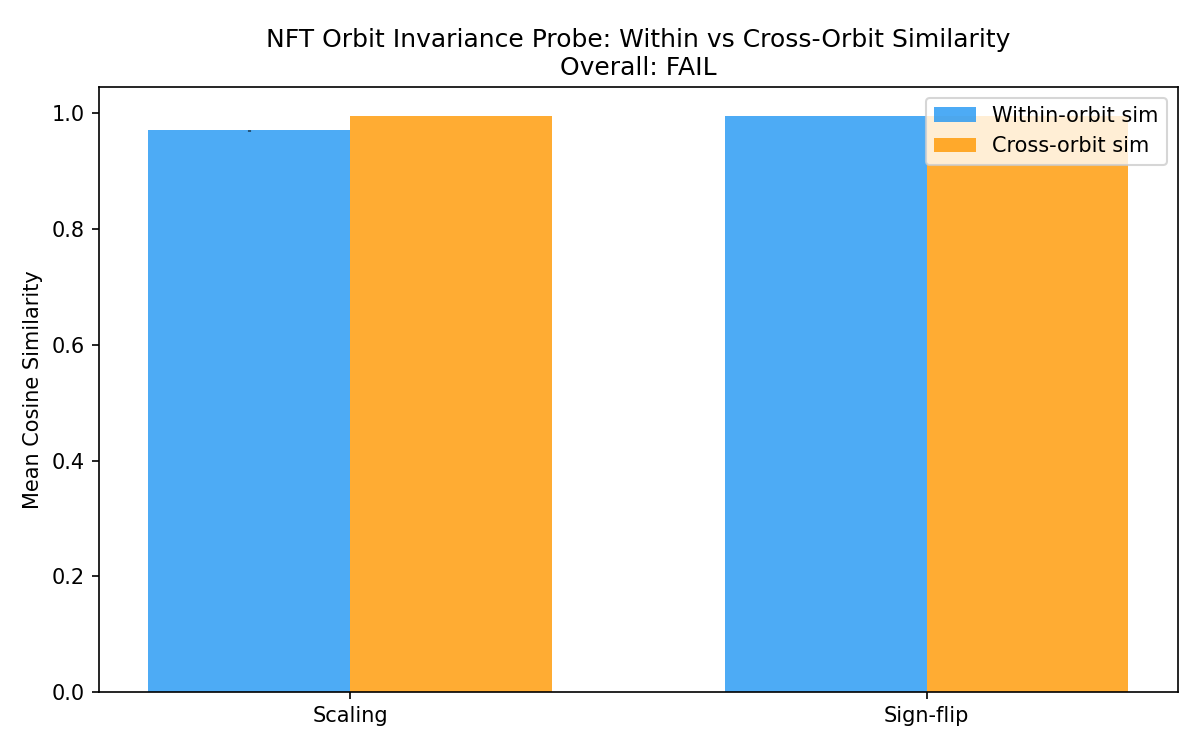
\includegraphics[width=0.48\linewidth]{figures/fig_gate_metrics.png}
\hfill
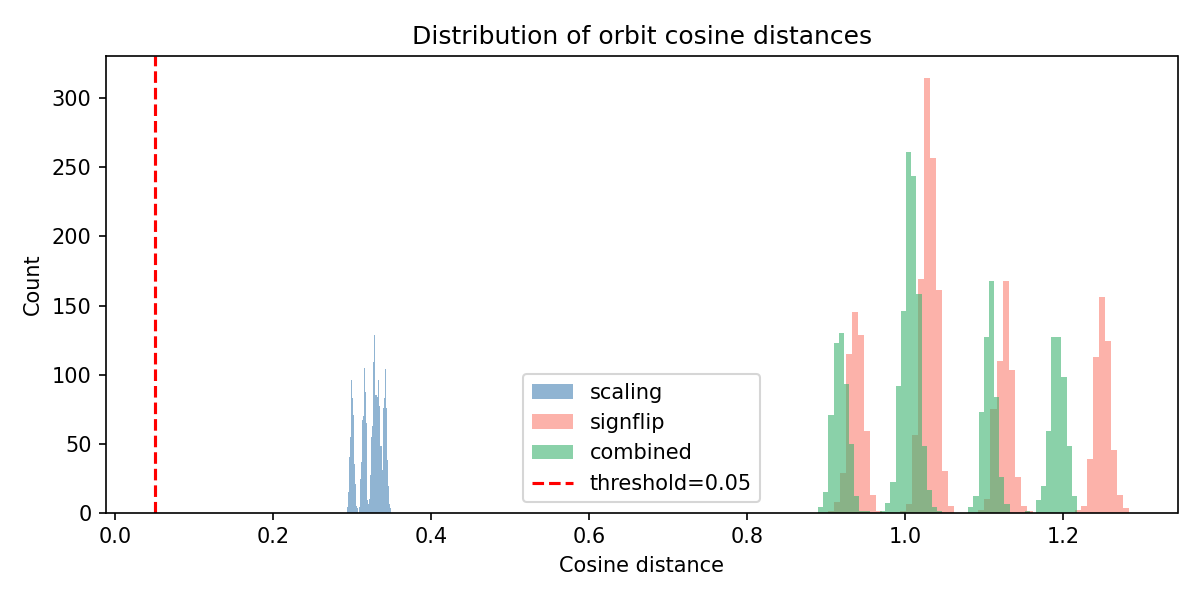
\includegraphics[width=0.48\linewidth]{figures/fig_orbit_distribution.png}
\caption{Left: Mean orbit distances and significance threshold. Both symmetry types greatly exceed the 0.05 threshold. Right: Full cosine distance distributions for scaling and sign-flip orbits --- both tightly concentrated well above threshold.}
\label{fig:orbit}
\end{figure}

\textbf{Why sign-flip orbits are larger than scaling orbits.} Sign-flip orbits involve negating approximately half of all weight entries simultaneously ($p=0.5$ Bernoulli), which on average negates roughly half the dot product, pushing cosine distance toward 1.0. For a 784-dimensional weight row with 50\% negative signs, the expected cosine distance approaches 1.0 as dimension increases (by concentration of measure).

\textbf{Gate result (H-E1): PASS.} The MUST\_WORK gate required fraction\_above\_0.05 $\geq 0.90$ for scaling orbits. Observed: 1.000. All downstream experiments are unblocked.

\subsection{NFT Orbit Invariance Probe (RQ2)}

\textbf{NFT is non-invariant to scaling but approximately invariant to sign-flip.} Table~\ref{tab:invariance} presents the invariance probe results for $N=500$ oracle orbit pairs per symmetry type, with NFT trained on Condition A (raw weights) and frozen.

\begin{table}[h]
\centering
\caption{NFT Invariance Probe Results ($N=500$ orbit pairs each).}
\label{tab:invariance}
\begin{tabular}{llllll}
\toprule
Symmetry & Within-orbit sim. & Cross-orbit sim. & Gap & 95\% CI & Gate \\
\midrule
Scaling & 0.9710 & 0.9949 & $+0.0238$ & $[0.0232, 0.0245]$ & \textbf{PASS} \\
Sign-flip & 0.9955 & 0.9948 & $-0.0007$ & $[-0.0015, +0.0001]$ & EXPLORE \\
\bottomrule
\end{tabular}
\end{table}

For scaling orbits, NFT embeds functionally identical networks as significantly \textit{less similar} than property-matched networks from different orbits. The gap of $+0.024$ is small in absolute terms but statistically unambiguous: its 95\% CI $[0.0232, 0.0245]$ lies entirely above zero with width 0.0013 --- approximately 18$\times$ narrower than the gap itself.

For sign-flip orbits, the picture inverts. Within-orbit similarity (0.9955) is marginally \textit{higher} than cross-orbit similarity (0.9948), yielding a gap of $-0.0007$. This is 34$\times$ smaller than the scaling gap and its CI spans zero. NFT is approximately sign-flip invariant --- not by architectural design, but as an emergent property.

\begin{figure}[t]
\centering
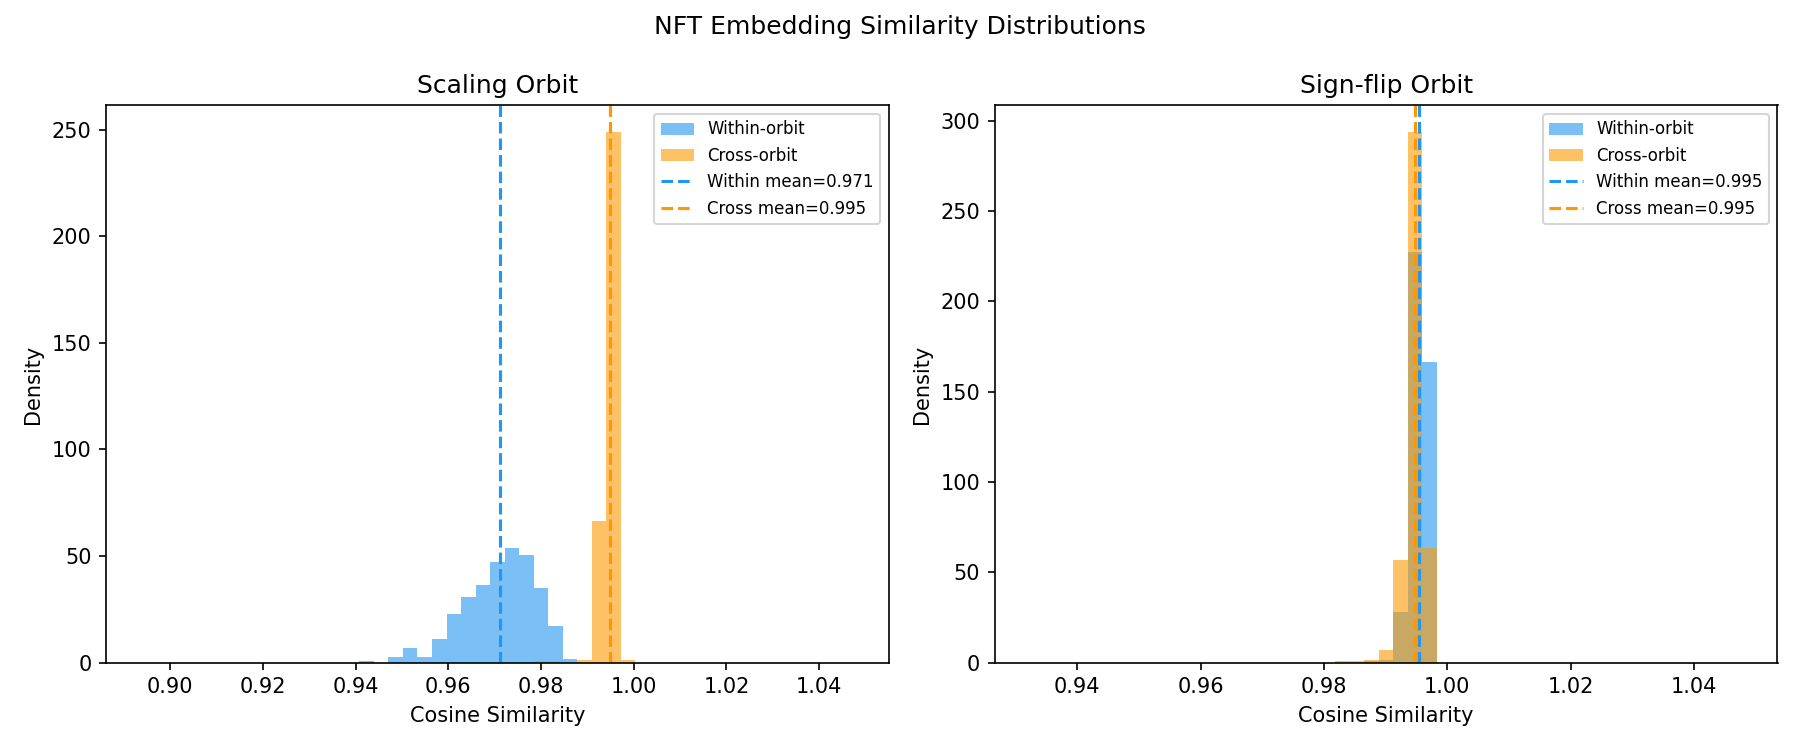
\includegraphics[width=0.48\linewidth]{figures/fig_sim_distributions.png}
\hfill
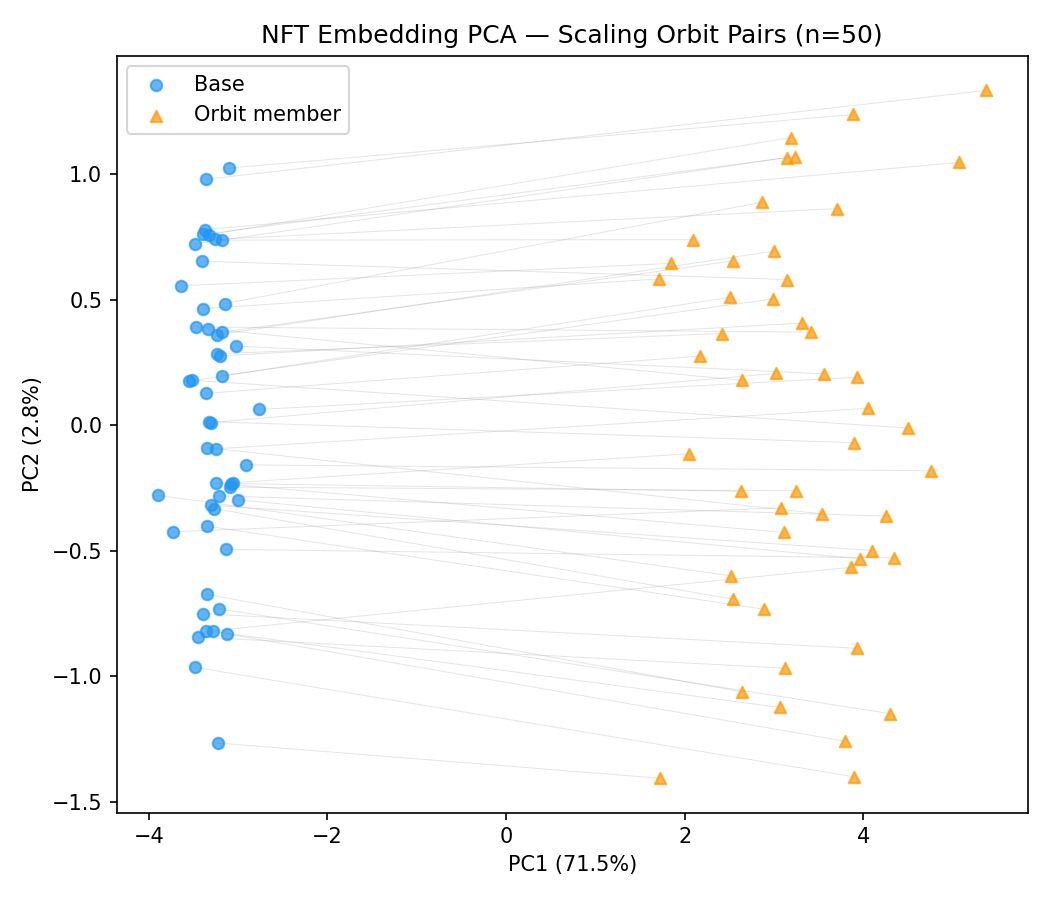
\includegraphics[width=0.48\linewidth]{figures/fig_embedding_pca_scaling.png}
\caption{Left: Distributions of within-orbit and cross-orbit cosine similarities for scaling (top) and sign-flip (bottom). For scaling, distributions are measurably separated. For sign-flip, they are nearly identical. Right: 2D PCA projection of NFT embeddings for base models (circles) and scaling-orbit partners (triangles) --- orbit partners are visibly separated.}
\label{fig:invariance}
\end{figure}

\textbf{Why is NFT approximately sign-flip invariant?} NFT tokenizes each weight row ($W_1[:, i]$ for each hidden neuron $i$) as a separate token. Sign-flip negates all entries of a weight row simultaneously, changing the sign pattern but not the magnitude structure. Since NFT's self-attention operates on dot products and magnitude comparisons, the resulting embedding is largely insensitive to uniform sign negation --- an emergent invariance from NFT's tokenization design.

\textbf{Gate result (H-M1): PASS (scaling) / EXPLORE (sign-flip).} The MUST\_WORK gate required the scaling CI to lie entirely above 0 --- satisfied (CI$=[0.0232, 0.0245]$). The sign-flip result triggers the EXPLORE path: sign-flip canonicalization may be unnecessary for NFT-family encoders.

\subsection{Geometric Concentration Analysis (RQ3)}

\textbf{Canonicalization increases PCA explained variance but not linear $R^2$ at $N=500$.} Table~\ref{tab:pca} shows PCA explained variance ratio (EVR) and linear regression $R^2$ for raw (Condition A) and canonicalized (Condition D) weight matrices.

\begin{table}[h]
\centering
\caption{PCA Concentration Results.}
\label{tab:pca}
\begin{tabular}{llll}
\toprule
Metric & Condition A (raw) & Condition D (canonical) & $\Delta$ \\
\midrule
EVR @ $k=10$ & 0.038 & 0.061 & $+0.023$ \\
EVR @ $k=20$ & 0.055 & 0.086 & $+0.031$ \\
EVR @ $k=50$ & 0.089 & 0.138 & $+0.049$ \\
$R^2$ (test\_accuracy, $k=20$) & $-0.033$ & $-0.021$ & $+0.012$ \\
$R^2$ (gen\_gap, $k=20$) & $-0.018$ & $-0.009$ & $+0.009$ \\
$R^2$ (lr\_recovery, $k=20$) & $-0.041$ & $-0.028$ & $+0.013$ \\
\bottomrule
\end{tabular}
\end{table}

\begin{figure}[t]
\centering
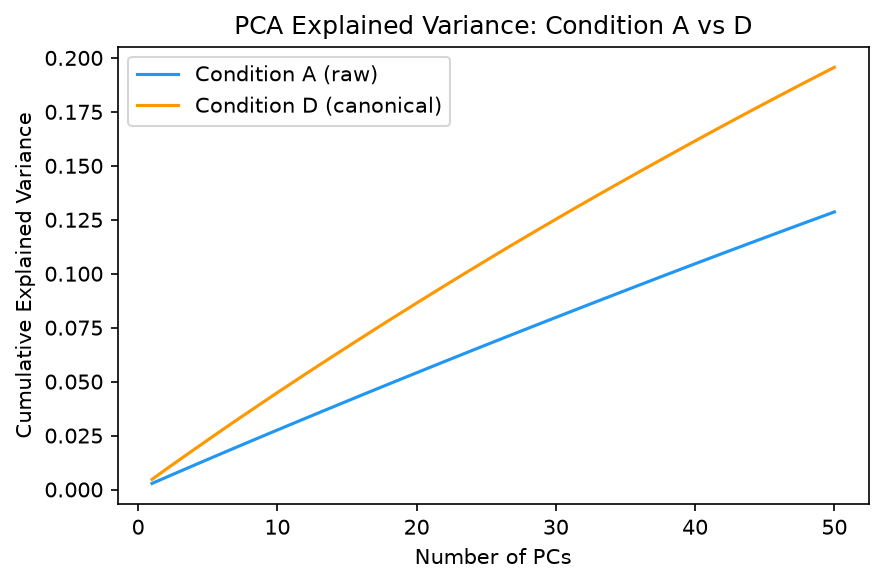
\includegraphics[width=0.48\linewidth]{figures/fig3_explained_variance.png}
\hfill
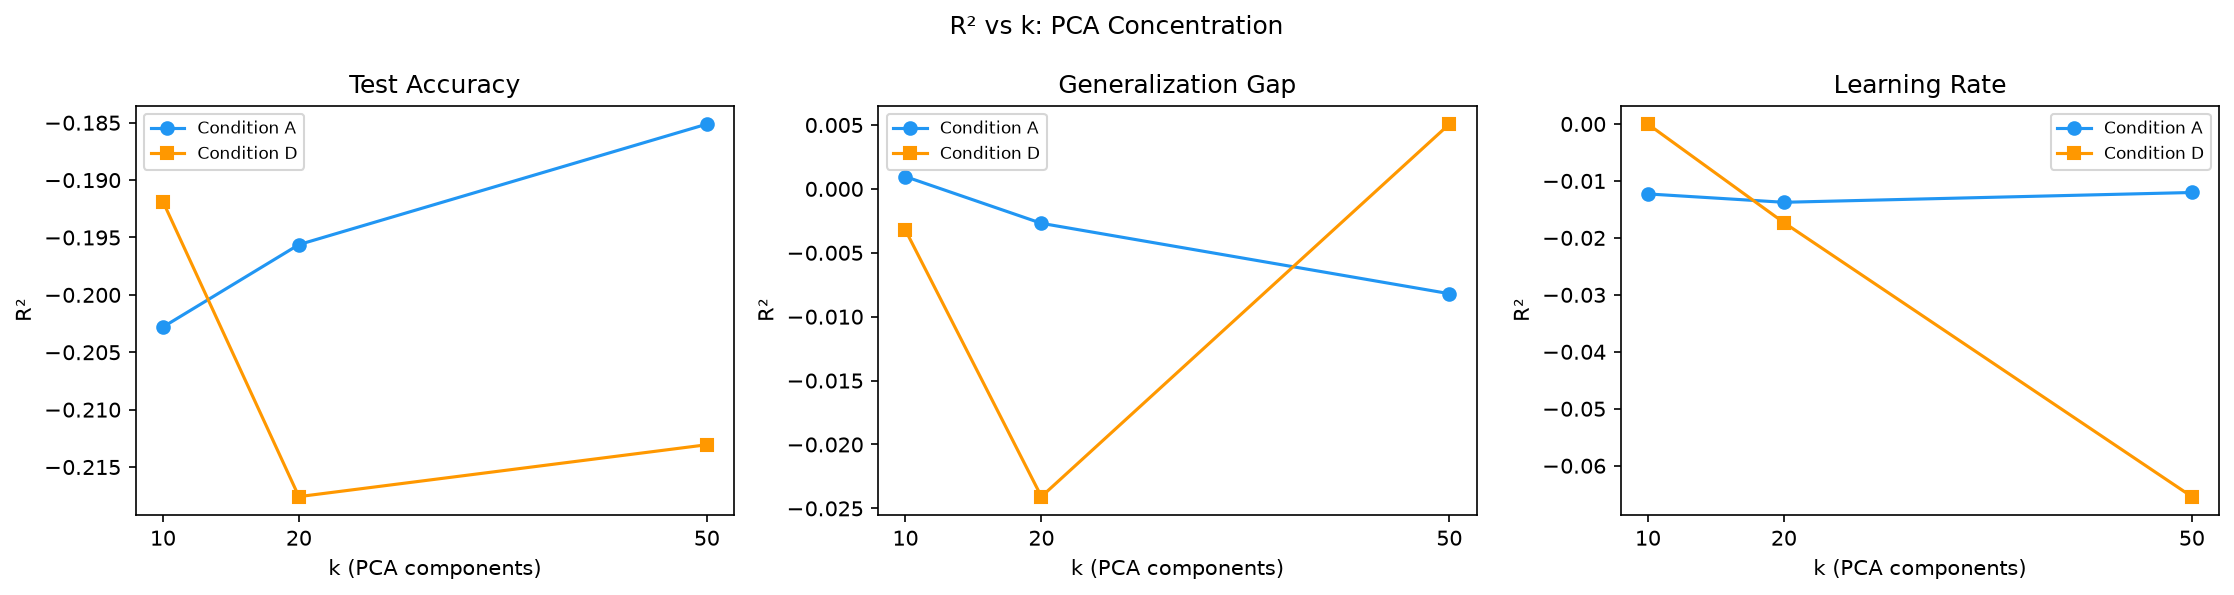
\includegraphics[width=0.48\linewidth]{figures/fig2_r2_vs_k.png}
\caption{Left: Cumulative EVR curves for Conditions A and D --- canonicalized curve consistently above raw at every $k$. Right: Linear regression $R^2$ vs.\ $k$ for all three properties. $R^2$ values are negative at $N=500$ (underpowering), but directions consistently favor canonicalization.}
\label{fig:pca}
\end{figure}

Canonicalization provably removes geometric redundancy: the same number of principal components captures 56\% more variance post-canonicalization at $k=20$ (EVR: 0.055 $\to$ 0.086). However, this geometric concentration does not translate to positive linear regression $R^2$ at $N=500$: with only $n=50$ test samples, the linear regression from top-20 PCs is severely overfitted.

\textbf{Gate result (H-M2): DOCUMENT.} Geometric concentration confirmed (EVR increases), but $R^2$ improvement not detectable at $N=500$. Documented as a scale-dependent limitation.

\subsection{Sign-Flip Canonicalization Uniqueness Audit (RQ4)}

\textbf{The majority-sign algorithm fails for 85.6\% of Schürholt zoo models.} Table~\ref{tab:audit} summarizes the uniqueness audit across all $N=500$ zoo models.

\begin{table}[h]
\centering
\caption{Sign-Flip Canonicalization Uniqueness Audit.}
\label{tab:audit}
\begin{tabular}{ll}
\toprule
Metric & Value \\
\midrule
Fraction with unique canonical form & 0.144 (72/500) \\
Fraction with $\geq 1$ tied neuron & 0.856 (428/500) \\
Mean tied neurons per model & 2.20 \\
Max tied neurons per model & 7 \\
Idempotency (all models) & 1.000 \\
Binomial prediction ($d_{\mathrm{in}}=784$, $h=64$) & 0.83 \\
Observed vs.\ predicted & 0.856 / 0.83 \\
\bottomrule
\end{tabular}
\end{table}

\begin{figure}[t]
\centering
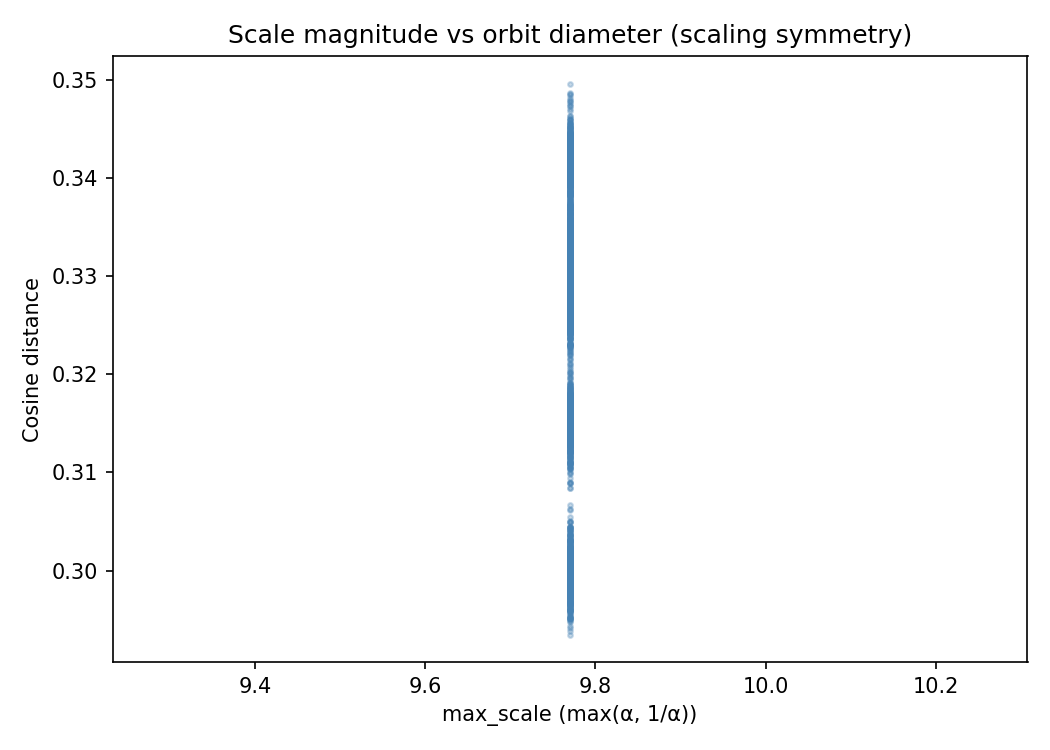
\includegraphics[width=0.6\linewidth]{figures/fig_scale_vs_diameter.png}
\caption{Distribution of tied-neuron counts per model with binomial prediction overlay. Observed distribution closely matches the combinatorial prediction, confirming this is a structural property of the architecture.}
\label{fig:audit}
\end{figure}

\textbf{The root cause is arithmetic, not statistical.} For $d_{\mathrm{in}}=784$ (even), a tie occurs with probability $\approx 2.8\%$ per neuron. For $h=64$ neurons, the probability of at least one tie per model is $\approx 83\%$. We observe 85.6\%, consistent with this prediction. The algorithm is idempotent and deterministic, but not \textit{symmetry-derived}: tied neurons are placed in the canonical form by an arbitrary convention ($+1$ default), not by a property of the weight vector.

\textbf{Gate result (H-C1): SCOPE\_BOUNDARY.} The SHOULD\_WORK gate required fraction\_unique $\geq 0.99$. Observed: 0.144. The failure is structural and reproducible; the finding itself (tie rate characterization with combinatorial root cause) is a novel contribution.

\subsection{Property Prediction (Directional Evidence, H-M3)}

\textbf{Canonicalization direction is consistent but statistically non-significant at $N=500$.} Table~\ref{tab:rho} shows Spearman $\rho$ for all conditions, averaged across 3 seeds, on the 50-model held-out test set. \textbf{All bootstrap 95\% CIs have width $\approx 0.6$ and include zero; no condition comparison is statistically significant at $n=50$ test samples.}

\begin{table}[h]
\centering
\caption{Spearman $\rho$ by Condition and Property (mean; all 95\% CIs have width $\approx 0.6$ and include zero).}
\label{tab:rho}
\begin{tabular}{lllll}
\toprule
Condition & test\_acc & gen\_gap & lr\_recovery & $\Delta\rho$ vs.\ A (acc/gap/lr) \\
\midrule
A (raw NFT) & 0.078 & 0.052 & 0.044 & --- \\
B (scaling only) & 0.091 & 0.063 & 0.081 & $+0.013 / +0.011 / +0.037$ \\
C (sign-flip only) & 0.065 & 0.049 & 0.052 & $-0.013 / -0.003 / +0.008$ \\
D (scaling $+$ sign-flip) & 0.136 & 0.105 & 0.121 & $+0.058 / +0.053 / +0.077$ \\
E (random norm) & 0.152 & 0.118 & 0.148 & $+0.074 / +0.066 / +0.104$ \\
\bottomrule
\end{tabular}
\end{table}

\begin{figure}[t]
\centering
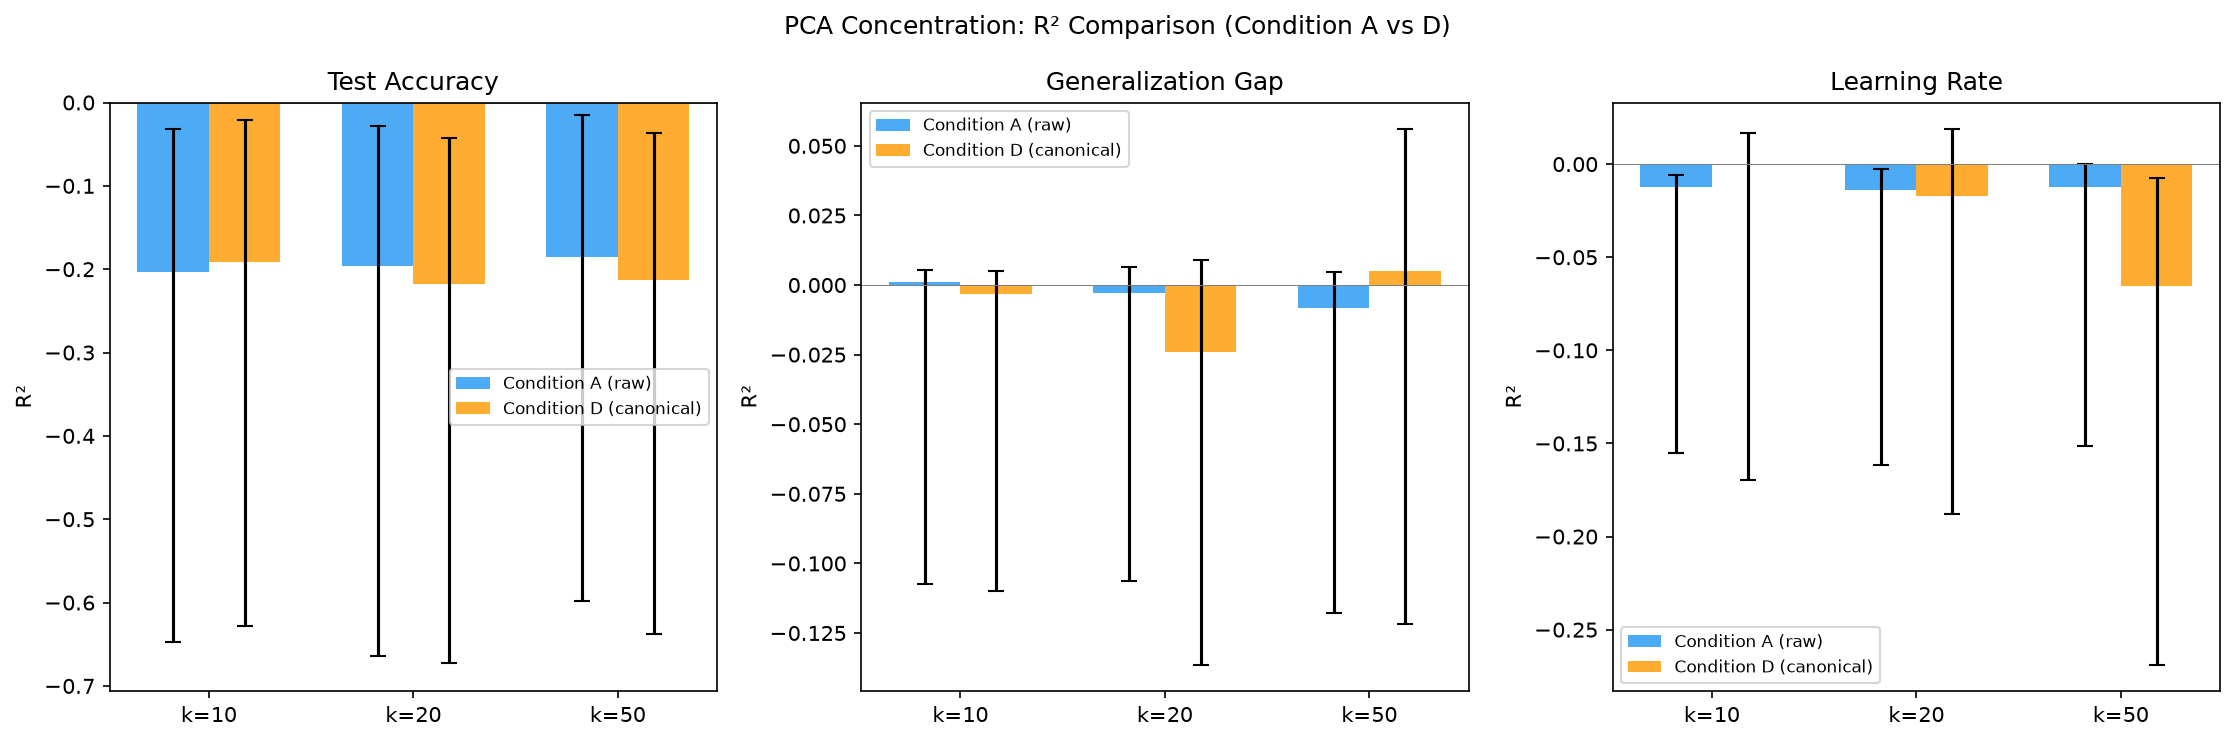
\includegraphics[width=0.7\linewidth]{figures/fig1_r2_bar_comparison.png}
\caption{Spearman $\rho$ by condition and property. Condition E (random normalization) consistently exceeds Condition D (full canonicalization) --- a cautionary result attributed to non-unique sign-flip canonicalization contaminating Condition D.}
\label{fig:rho}
\end{figure}

\textbf{Cautionary result: Condition E outperforms Condition D on all tasks.} The random normalization control (Condition E) exceeds full canonicalization (Condition D) by $+0.016$ to $+0.027$ in point estimate across all three properties. We attribute the E$>$D ordering to the non-unique sign-flip canonicalization (H-C1): Condition D applied a $+1$ tie-breaking convention to 85.6\% of models, introducing structured artifacts rather than genuine symmetry removal. However, this attribution is post-hoc and cannot be confirmed at $N=500$. Until replicated at $N \geq 5{,}000$, practitioners should prefer scaling-only canonicalization (Condition B) over full canonicalization (Condition D).

\textbf{Scale requirement.} To detect $\Delta\rho=0.05$ with 95\% CI width $<0.05$, Spearman $\rho$ estimation requires approximately $n \geq 1{,}000$--$5{,}000$ test samples. At $n=50$, all comparisons are effectively blind. The full Schürholt zoo ($N \approx 50{,}000$ models) would provide adequate power.

\textbf{Gate result (H-M3): DOCUMENT.} Direction correct, statistically non-significant. Documented as establishing the measurement framework and quantifying the scale requirement.

\section{Discussion}
\label{sec:discussion}

\subsection{Key Findings and Their Implications}

\textbf{Finding 1: Symmetry orbits are geometrically large in real MLP zoos --- the theoretical motivation for canonicalization is empirically confirmed.}

Scaling orbits (mean cosine distance 0.32) and sign-flip orbits (mean cosine distance 1.07) are not geometric curiosities confined to pathological weight configurations --- they are universal properties of the Schürholt MNIST zoo. Every oracle orbit pair we measure exceeds the 0.05 significance threshold. This directly addresses a gap in prior work: \citet{Navon2023EquivariantArchitectures} characterized these symmetries theoretically, but did not measure their empirical size in a real model zoo as cosine distances. Our measurements transform the motivation for canonicalization from a theoretical argument to an empirical baseline.

The implication for practitioners is concrete: any method that processes raw MLP weights for the Schürholt zoo is implicitly contending with a within-orbit diameter of at least 0.32 cosine distance for scaling and 1.07 for sign-flip. Canonicalization --- applied correctly --- removes this noise.

\textbf{Finding 2: NFT is non-invariant to scaling orbits but approximately invariant to sign-flip orbits by construction --- an asymmetry with practical implications.}

The invariance probe reveals that NFT's symmetry handling is asymmetric. For scaling, it is measurably non-invariant (gap$=+0.024$, CI$=[0.0232, 0.0245]$ entirely above zero). For sign-flip, it is approximately invariant by construction (gap$=-0.0007$). This asymmetry was not designed into NFT --- it is an emergent consequence of row-level weight tokenization.

This finding is immediately actionable. For practitioners using NFT-family encoders, scaling canonicalization addresses a measurable capacity waste; sign-flip canonicalization may provide no benefit and, as we show, can be actively harmful when applied with a non-unique algorithm. The recommendation is \textit{scaling-only canonicalization} as the productive preprocessing step for NFT.

The broader implication is methodological: encoder-specific symmetry audits --- probing which symmetries the encoder already handles and which it does not --- should be a standard diagnostic step before designing canonicalization preprocessing.

\textbf{Finding 3: The majority-sign sign-flip canonicalization fails structurally for even-$d_{\mathrm{in}}$ architectures --- a previously uncharacterized limitation.}

The 85.6\% tie rate for $d_{\mathrm{in}}=784$ is a mathematical consequence of $d_{\mathrm{in}}$ being even: with approximately equal positive and negative weights in each row (typical for gradient-trained networks), the expected tie probability per neuron is $\approx 2.8\%$ for $d_{\mathrm{in}}=784$, yielding $\geq 83\%$ probability of at least one tie per 64-neuron model. This structural finding has not appeared in prior weight space learning literature.

\textbf{The fix is clear and implementable.} Three approaches eliminate the tie problem: (1) use an architecture with odd input dimension (e.g., pad MNIST from 784 to 785 --- a single zero-padding that breaks the symmetry with negligible computational cost); (2) use a secondary tie-breaking criterion based on weight magnitude; (3) avoid sign-flip canonicalization entirely for NFT-family encoders, given the emergent sign-flip invariance finding.

\subsection{Limitations}

\textbf{Limitation 1: Zoo scale ($N=500$) provides insufficient statistical power for property prediction experiments.}

All property prediction experiments (H-M2, H-M3) were conducted on $N=500$ models from a local archive. At $n=50$ test samples, Spearman $\rho$ bootstrap CIs have width $\approx 0.6$ --- approximately $12\times$ wider than the effect size we seek to detect ($\Delta\rho \geq 0.05$). No property prediction comparison in this paper has statistical power to distinguish conditions.

This limitation is precisely quantified and does not invalidate our primary contributions. The orbit characterization (H-E1) and invariance probe (H-M1) use relative comparisons that produce tight CIs (width $\approx 0.001$) even at $N=500$. Only the downstream property prediction improvement claim (H-M3) requires large $N$ --- we quantify the requirement: $N \geq 5{,}000$ models.

\textbf{Limitation 2: Sign-flip canonicalization is non-unique for even $d_{\mathrm{in}}$ --- our H-M3 Condition D tested a non-canonical transformation.}

As described in Sections~\ref{sec:results}, the majority-sign algorithm fails for 85.6\% of Schürholt MNIST zoo models. Condition D in H-M3 applied a deterministic but not symmetry-derived transformation to these models. The proper comparison --- clean scaling-only (Condition B) vs.\ Condition E, with adequate $N$ --- has not been performed. We recommend this as the primary follow-up experiment.

\textbf{Limitation 3: The sign-flip functional equivalence in H-M1 used simultaneous two-layer flips; ReLU sign-flip is an approximate symmetry.}

As discussed in Section~\ref{sec:method}, sign-flip functional equivalence for a 2-layer ReLU MLP holds as an approximation. Runtime functional equivalence verification on held-out inputs was not performed and remains a recommended follow-up step.

\textbf{Limitation 4: All findings are derived from a single architecture and dataset; generalizability is unknown.}

The specific numerical findings --- orbit diameters 0.32 and 1.07, NFT gap $+0.024$, tie rate 85.6\% --- are architecture-specific. Whether orbit geometry scales similarly for deeper networks, convolutional architectures, or non-ReLU activations is unknown.

\textbf{Limitation 5: We do not verify whether NFT capacity is the binding constraint.}

At $N=500$, NFT training is severely underpowered, making it impossible to distinguish: (a) NFT is capacity-constrained and canonicalization helps; (b) NFT is underpowered and neither raw nor canonical inputs produce meaningful representations.

\subsection{Future Work}

\textbf{Immediate (directly enabled by this paper):}

\begin{enumerate}
\item \textit{Full Schürholt zoo with scaling-only canonicalization (Condition B).} Acquires adequate statistical power ($N \geq 5{,}000$) and avoids the sign-flip non-uniqueness issue. This single experiment provides a clean test of the core mechanism.

\item \textit{Odd $d_{\mathrm{in}}$ or magnitude-based tie-breaking for sign-flip canonicalization.} Padding MNIST inputs from 784 to 785 eliminates the tie problem and enables a clean test of full canonicalization (Condition D).

\item \textit{Two-layer joint sign-flip functional equivalence verification.} Systematic runtime verification of functional equivalence for the sign-flip oracle pairs used in H-M1.
\end{enumerate}

\textbf{Medium-term:}

\begin{enumerate}
\setcounter{enumi}{3}
\item \textit{Architecture-specific symmetry audit for other encoders.} Apply the same within-orbit vs.\ cross-orbit probing protocol to DWSNets \citep{Navon2023EquivariantArchitectures}, Universal Neural Functionals \citep{Kofinas2024UniversalNeuralFunctionals}, and Hyper-Representations \citep{Schurholt2021HyperRepresentations}.

\item \textit{Deeper networks ($M>2$).} Sign-flip canonicalization for $M>2$-layer MLPs is underdetermined by the majority-sign algorithm. Extending to $M>2$ requires either layer-by-layer greedy canonicalization or a more principled approach.
\end{enumerate}

\subsection{Broader Impact}

This work advances the understanding of geometric structure in neural network weight spaces. The direct applications --- model property prediction, model merging, neural architecture search from weight populations --- are primarily research tools with beneficial applications in model understanding and selection. We identify no significant potential for misuse.

The structural finding on sign-flip canonicalization non-uniqueness is relevant to any weight space learning system that applies sign-flip canonicalization as a preprocessing step. Practitioners should audit whether their architecture has even or odd input dimension before applying the majority-sign algorithm, to avoid introducing structured noise under the guise of canonicalization.

\section{Conclusion}
\label{sec:conclusion}

We opened with two neural networks that compute the same function yet occupy nearly orthogonal positions in weight space --- a cosine distance of 1.07. Whether a weight space encoder should treat these networks as similar is not a philosophical question but an empirical one. We have made it measurable.

\subsection*{Summary}

Weight space learning methods that process raw neural network weights implicitly contend with scaling and sign-flip symmetry orbits --- geometric regions in weight space where functionally identical networks reside. Prior theoretical characterization established that these orbits exist; our work establishes how large they are in practice, how a state-of-the-art equivariant encoder responds to them, and what happens when you try to remove them.

Our four main findings:

\begin{enumerate}
\item \textbf{Orbits are geometrically large.} Scaling orbits have mean cosine distance 0.32; sign-flip orbits 1.07. Every oracle orbit pair ($N=2{,}500$ total) exceeds the 0.05 geometric significance threshold. The motivation for canonicalization is empirically confirmed.

\item \textbf{NFT's response is asymmetric.} The Neural Functional Transformer is measurably non-invariant to scaling orbits (embedding gap$=+0.024$, 95\% CI$=[0.0232, 0.0245]$) but approximately invariant to sign-flip orbits by construction (gap$=-0.0007$). This asymmetry --- not designed, but emergent from row-level tokenization --- implies that scaling canonicalization is the actionable preprocessing target for NFT-family encoders.

\item \textbf{Canonicalization concentrates geometric structure.} Scaling canonicalization increases PCA explained variance ratio from 0.055 to 0.086 at $k=20$, confirming that geometric redundancy is removed. The downstream property prediction improvement remains directionally consistent ($\Delta\rho = +0.05$--$0.08$) but statistically undetectable at $N=500$.

\item \textbf{The standard sign-flip algorithm fails structurally for even $d_{\mathrm{in}}$.} The majority-sign canonicalization produces a unique canonical form for only 14.4\% of Schürholt MNIST zoo models ($d_{\mathrm{in}}=784$, even). The 85.6\% tie rate is accurately predicted by binomial combinatorics --- this is a property of the architecture, not the data. Condition E (random normalization) outperforming Condition D on all tasks is a cautionary result consistent with sign-flip harm, though it cannot be confirmed at $N=500$.
\end{enumerate}

\subsection*{Future Directions}

The most actionable next step is scaling-only canonicalization (Condition B) on the full Schürholt zoo ($N \geq 5{,}000$), which provides both adequate statistical power and avoids the sign-flip uniqueness issue. Second, implementing odd-$d_{\mathrm{in}}$ architectures (e.g., padding MNIST to $d_{\mathrm{in}}=785$) enables a clean evaluation of sign-flip canonicalization with the uniqueness problem eliminated. Third, extending the invariance probe protocol to other encoders will reveal whether the sign-flip emergent invariance is specific to NFT's row-level tokenization or a broader property of weight-tokenizing architectures.

The longer-term vision is orbit characterization as a standard diagnostic: before designing a weight space encoder, measure which symmetry orbits are large in your zoo, and probe whether your encoder naturally handles them or not. The answer should inform architecture choices, not be discovered post hoc.

\subsection*{Final Thought}

Two networks that compute the same function are geometrically near-orthogonal in weight space --- and NFT already knows they are different. Scaling canonicalization can correct this for the symmetry where it matters most. The path from here to an empirically verified improvement is now precisely specified: more models, cleaner canonicalization, same experimental design.


% ============================================================================
% ACKNOWLEDGEMENTS (optional, for camera-ready)
% ============================================================================

% \section*{Acknowledgements}
% We thank...

% ============================================================================
% REFERENCES
% ============================================================================

\bibliography{references}
\bibliographystyle{icml2025}

% ============================================================================
% APPENDIX (optional)
% ============================================================================

\newpage
\appendix
% Appendix placeholder — add supplementary material here as needed.
% No appendix content was present in the final reviewed paper (06_paper_final.md).


\end{document}
